\documentclass{article}

\usepackage{lipsum}
\usepackage[margin=1.2in]{geometry}
\usepackage{titlesec}
\usepackage{graphicx}
\usepackage{amsmath}

\newcommand{\code}{\texttt}
\newcommand{\norm}[1]{\left\lVert#1\right\rVert}

\usepackage{siunitx} % Required for alignment

\sisetup{
  round-mode          = places, % Rounds numbers
  round-precision     = 2, % to 2 places
}

% Specify images directory
\graphicspath{ {./report-images/} }

% Header and Footer stuff
\usepackage{fancyhdr}
\pagestyle{fancy}
\fancyhead{}
\fancyfoot{}
\fancyfoot[R]{ \thepage\ }
\renewcommand{\headrulewidth}{0pt}
\renewcommand{\footrulewidth}{0pt}
\newcommand{\sectionbreak}{\clearpage}
\setlength{\parindent}{0pt}

%

\begin{document}

%----------------------------------------------------------------------------------------
%	TITLE PAGE
%----------------------------------------------------------------------------------------

\begin{titlepage} % Suppresses displaying the page number on the title page and the subsequent page counts as page 1
	\newcommand{\HRule}{\rule{\linewidth}{0.5mm}}% Defines a new command for horizontal lines, change thickness here
	
	\center % Centre everything on the page
	
	%------------------------------------------------
	%	Headings
	%------------------------------------------------
	
	\textsc{\Large Systems of Linear Equations}\\[0.5cm] % Major heading such as course name
	
	\textsc{\large Exercise 7}\\[0.5cm] % Minor heading such as course title
	
	%------------------------------------------------
	%	Title
	%------------------------------------------------
	
	\HRule\\[0.6cm]
	
	{\huge\bfseries Solving a Linear System with LU Decomposition}\\[0.25cm] % Title of your document
	
	\HRule\\[1.5cm]
	
	%------------------------------------------------
	%	Author(s)
	%------------------------------------------------
	
	\begin{minipage}{0.4\textwidth}
		\begin{flushleft}
			\large
			\textit{Author}\\
			\textsc{Cesare De Cal} % Your name
		\end{flushleft}
	\end{minipage}
	~
	\begin{minipage}{0.4\textwidth}
		\begin{flushright}
			\large
			\textit{Professor}\\
			\textsc{Annie Cuyt}\\ % Supervisor's name
			[0.25cm]
			\textit{Assistant Professor}\\
			\textsc{Ferre Knaepkens} % Supervisor's name

		\end{flushright}
	\end{minipage}
		
	\vfill\vfill\vfill
	
	{\large\today}
		
	\vfill
	
\end{titlepage}

%----------------------------------------------------------------------------------------

\section{Introduction}\label{sec:intro}
In this exercise I am going to use solve a linear system $A\vec{x}=\vec{y}$ using LU decomposition. The goal is to verify that first element of the unknowns vector, $x_{1}$, will contain an approximation of $e - 2$.\\

As we've seen in class, there are multiple ways of solving a linear system $AX=B$. Assume $A$ is a $n\times n$ square matrix, $B$ is a "constant" term matrix $n\times h$, and $X$ is a $n\times h$ unknown matrix. To solve for $X$, we could compute the inverse of $A$ and find $x=A^{-1}y$. We've seen that this approach, however, requires more computations than necessary and returns a less accurate result.\\

On the other hand, the LU decomposition technique is a way to represent the matrix A in the form of simpler matrices, $L$ and $U$ (lower triangular and upper triangular matrices, respectively):
$$PA=LU$$

This method uses forward substitution (solving for $Y$ from $LY=B$) and backward substitution (solving for $X$ from $UX = Y$). I'll be specifically solving the system by using Gaussian Elimination with partial pivoting, which reduces round-offs errors compared to its naive implementation. I'll also be calculating the error and the condition number as the variable $n$ increases, and plot the results.

\section{Tools}
The following programming language and libraries have been used in this exercise:
\begin{itemize}
  \item C
  \item GSL (GNU Scientific Library)
\end{itemize}
The following double-precision GSL data types have been used in the exercise:
\begin{itemize}
  \item \code{gsl\_vector}
  \item \code{gsl\_matrix}
  \item \code{gsl\_permutation}
\end{itemize}
The following GSL methods have been used in the exercise:
\begin{itemize}
  \item \code{gsl\_matrix\_alloc(size1, size2)}
  \item \code{gsl\_matrix\_set\_zero(matrix)}
  \item \code{gsl\_matrix\_set(matrix, row, column, value)}
  \item \code{gsl\_matrix\_get(matrix, row, column)}
  \item \code{gsl\_vector\_alloc(size)}
  \item \code{gsl\_vector\_set\_zero(vector)}
  \item \code{gsl\_vector\_set(vector, index, value)}
  \item \code{gsl\_vector\_get(vector, index)}
  \item \code{gsl\_matrix\_memcpy(matrixToCopyFrom, matrix)}
  \item \code{gsl\_linalg\_SV\_decomp(A, V, S, workspaceVector)}
  \item \code{gsl\_vector\_minmax(vector, minInVector, maxInVector)}
\end{itemize}
In order to factorize a matrix into the LU decomposition, and then solve the square system $Ax=y$ using the decomposition of A, I've used the following methods:
\begin{itemize}
  \item \code{gsl\_linalg\_LU\_decomp(A, permutation, signum)}
  \item \code{gsl\_linalg\_LU\_solve(LU, permutation, b, x)}
  \item \code{gsl\_permutation\_alloc(size)}
\end{itemize}
  
\section{Solving the linear system}
In order to solve the system $Ax=y$, I first need to build the matrix A by understanding how it's build. The requirements are to build a tridiagonal matrix with the values $-1$ on the adjacent upper diagonal, the entries $+1$ on the adjacent lower diagonal, and on the main diagonal the values $b_{i}$, with $i = 1, \ldots, n$ given by

$$b_i =\frac{2(i+1)}{3},\quad i + 1= 3, 6, 9,\ldots$$
$$b_i =1,\quad i + 1 = 2, 4, 5, 7, 8, \ldots$$

By looking closely at the first rule, we see that the $i+1$ are all multiples of 3 ($i+1 = 3*k$, for some $k$). Hence the $i$ are of the form $i = 3*k-1$, for some $k$. For $n = 5$, for example, this is what the matrix looks like:
$$
\begin{bmatrix}
1.0000000000 & -1.0000000000 & 0.0000000000 & 0.0000000000 & 0.0000000000 \\
1.0000000000 & 2.0000000000 & -1.0000000000 & 0.0000000000 & 0.0000000000 \\
0.0000000000 & 1.0000000000 & 1.0000000000 & -1.0000000000 & 0.0000000000 \\ 
0.0000000000 & 0.0000000000 & 1.0000000000 & 1.0000000000 & -1.0000000000 \\ 
0.0000000000 & 0.0000000000 & 0.0000000000 & 1.0000000000 & 4.0000000000 \\\end{bmatrix}
$$

The coefficients matrix A is first allocated by using the \code{gsl\_matrix\_alloc} method, then I set all the elements to zero with \code{gsl\_matrix\_set\_zero} and finally nested \code{for} loops fill the diagonal values by checking the indexes. The coefficients reported above on the diagonal have 5 significant digits for improve the readability of this report.\\

I used the \code{gsl\_vector\_alloc} method to create an instance of the vector. All of its elements were set to zero by using \code{gsl\_vector\_set\_zero(vector)}. The exercise asks us to set the first element of the $y$ vector to one, so I used \code{gsl\_vector\_set(vector, 0, 1)} to assign the value 1 to index 0. For $n=5$, we have:
$$
\vec{y}=
\begin{bmatrix}
1.0000000000 \\
0.0000000000 \\
0.0000000000 \\
0.0000000000 \\
0.0000000000 \\
\end{bmatrix}
$$

Given the $Ax=y$ system, my goal is now to find the vector of the unknowns $x$. To do so, I first factorize $A$ into its LU decomposition by allocating a new matrix (so that the matrix which represents $A$ doesn't get overridden) using \code{gsl\_matrix\_memcpy} and then by calling \code{gsl\_linalg\_LU\_decomp}. This method utilizes Gaussian Elimination with partial pivoting to compute the decomposition. The following is the $LU$ matrix for $n=5$:
$$
LU=
\begin{bmatrix} 
1.0000000000 & -1.0000000000 & 0.0000000000 & 0.0000000000 & 0.0000000000\\ 
1.0000000000 & 3.0000000000 & -1.0000000000 & 0.0000000000 & 0.0000000000\\ 
0.0000000000 & 0.3333333333 & 1.3333333333 & -1.0000000000 & 0.0000000000\\ 
0.0000000000 & 0.0000000000 & 0.7500000000 & 1.7500000000 & -1.0000000000\\ 
0.0000000000 & 0.0000000000 & 0.0000000000 & 0.5714285714 & 4.5714285714\\
\end{bmatrix}
$$

I can now use the $LU$ matrix to solve the system by passing $LU$, $x$, a permutation structure \code{gsl\_permutation} (it contains the order of the indexes of the equations in the system to keep track of swapping) and $y$ to \code{gsl\_linalg\_LU\_solve}. This method uses forward and back-substitution to modify the contents of the $x$ vector given in input, which now looks like this (for $n=5$):

$$
\vec{x}=
\begin{bmatrix}
0.7187500000\\
-0.2812500000\\
0.1562500000\\
-0.1250000000\\
0.0312500000\\
\end{bmatrix}
$$

The first element looks contains an approximation of $e-2$. By increasing the size of the matrix $n$, $x_i$ becomes increasingly more precise. For $n=10$, for example:

$$
\vec{x}=
\begin{bmatrix}
0.7182817183\\
-0.2817182817\\
0.1548451548\\
-0.1268731269\\
0.0279720280\\
-0.0149850150\\
0.0129870130\\
-0.0019980020\\
0.0009990010\\
-0.0009990010\\
\end{bmatrix}
$$

Then, I calculate the condition number of the matrix $A$ of order $n$ which will give me a better idea if this is a well-conditioned or an ill-conditioned linear system. In GSL there is no direct function that calculates the condition number, but it's possible to use the ratio of the largest singular value of matrix A, $\sigma_n (A)$, to the smallest $\sigma_1 (A)$:

$$\kappa(A) := \frac{\sigma_n (A)}{\sigma_1 (A)}= \frac{\norm{A}}{\norm{A^{-1}}^{-1}}$$

I proceed to factorize $A$ into its singular value decomposition $SVD$ using the \code{gsl\_linalg\_SV\_decomp} method, and then use $\code{gsl\_vector\_minmax}$ to extract the minimum and maximum singular values out of the vector $S$ that contains the diagonal elements of the singular value matrix. \\

For $n=5$, the condition number is

$$\kappa(A) = \frac{\sigma_n (A)}{\sigma_1 (A)}= \frac{4.2051006107}{1.1426432872}=3.6801516779$$

For $n=10$, the condition number is

$$\kappa(A) = \frac{\sigma_n (A)}{\sigma_1 (A)}= \frac{6.2820508697}{1.1424251953}=5.4988728328$$

I calculate the error by subtracting the computed solution $x_{1}^{\ast}$ from the exact mathematical solution $\widetilde{x}$ (which can be obtained by using the $\code{M\_E}$ GSL constant minus 2).\\

Finally, I am now going to insert the $x_1$ component, the error, and the condition number for $n$ from 1 to 50 in the next page.
\begin{table*}[htb]
\centering % used for centering table
\begin{tabular}{c c c c} % centered columns (4 columns)
$n$ & $\widetilde{x}_1$ & $x_1^{\ast}- \widetilde{x}_1$ & $\kappa(A_n)$ \\ [0.65ex] % inserts table
%heading
\hline % inserts single horizontal line
01 & 1.000000000000000 & -0.281718171540955 & 1.000000000000000 \\
02 & 0.666666666666667 & 0.051615161792378 & 1.767591879243998 \\
03 & 0.750000000000000 & -0.031718171540955 & 2.561552812808830 \\
04 & 0.714285714285714 & 0.003996114173331 & 2.258696038055887 \\
05 & 0.718750000000000 & -0.000468171540955 & 3.680151677879533 \\
06 & 0.717948717948718 & 0.000333110510327 & 3.953864002022550 \\
07 & 0.718309859154930 & -0.000028030695884 & 3.847674609118915 \\
08 & 0.718279569892473 & 0.000002258566572 & 5.377037588047721 \\
09 & 0.718283582089552 & -0.000001753630507 & 5.727581839289335 \\
10 & 0.718281718281718 & 0.000000110177327 & 5.498872832802596 \\
11 & 0.718281835205993 & -0.000000006746947 & 7.100335770367996 \\
12 & 0.718281822943950 & 0.000000005515095 & 7.582164637599711 \\
13 & 0.718281828735696 & -0.000000000276651 & 7.195531702121659 \\
14 & 0.718281828445401 & 0.000000000013644 & 8.833149892375440 \\
15 & 0.718281828470584 & -0.000000000011539 & 9.488074730049041 \\
16 & 0.718281828458563 & 0.000000000000482 & 8.911558696408528 \\
17 & 0.718281828459065 & -0.000000000000020 & 10.571522848352377 \\
18 & 0.718281828459028 & 0.000000000000017 & 11.420182460381190 \\
19 & 0.718281828459046 & -0.000000000000001 & 10.638134074627382 \\
20 & 0.718281828459045 & -0.000000000000000 & 12.313199658654300 \\
21 & 0.718281828459045 & -0.000000000000000 & 13.368831043170752 \\
22 & 0.718281828459045 & -0.000000000000000 & 12.371078212614004 \\
23 & 0.718281828459045 & -0.000000000000000 & 14.057004794016557 \\
24 & 0.718281828459045 & -0.000000000000000 & 15.328629826257806 \\
25 & 0.718281828459045 & -0.000000000000000 & 14.108163769731830 \\
26 & 0.718281828459045 & -0.000000000000000 & 15.802262487437682 \\
27 & 0.718281828459045 & -0.000000000000000 & 17.296307059194255 \\
28 & 0.718281828459045 & -0.000000000000000 & 15.848093475192302 \\
29 & 0.718281828459045 & -0.000000000000000 & 17.548556166163607 \\
30 & 0.718281828459045 & -0.000000000000000 & 19.269757243499750 \\
31 & 0.718281828459045 & -0.000000000000000 & 17.590060434351265 \\
32 & 0.718281828459045 & -0.000000000000000 & 19.295614845413013 \\
33 & 0.718281828459045 & -0.000000000000000 & 21.247563252611098 \\
34 & 0.718281828459045 & -0.000000000000000 & 19.333536447042945 \\
35 & 0.718281828459045 & -0.000000000000000 & 21.043254557744980 \\
36 & 0.718281828459045 & -0.000000000000000 & 23.228736221077760 \\
37 & 0.718281828459045 & -0.000000000000000 & 21.078161279333553 \\
38 & 0.718281828459045 & -0.000000000000000 & 22.791345987426897 \\
39 & 0.718281828459045 & -0.000000000000000 & 25.212565199999691 \\
40 & 0.718281828459045 & -0.000000000000000 & 22.823680837817037 \\
41 & 0.718281828459045 & -0.000000000000000 & 24.539795564146115 \\
42 & 0.718281828459045 & -0.000000000000000 & 27.198526001362339 \\
43 & 0.718281828459045 & -0.000000000000000 & 24.569910774893234 \\
44 & 0.718281828459045 & -0.000000000000000 & 26.288533903235187 \\
45 & 0.718281828459045 & -0.000000000000000 & 29.186223702087091 \\
46 & 0.718281828459045 & -0.000000000000000 & 26.316714104617667 \\
47 & 0.718281828459045 & -0.000000000000000 & 28.037508462052152 \\
48 & 0.718281828459045 & -0.000000000000000 & 31.175355146341044 \\
49 & 0.718281828459045 & -0.000000000000000 & 28.063986916895736 \\
50 & 0.718281828459045 & -0.000000000000000 & 29.786678720210102 \\\hline %inserts single line
\end{tabular}
\end{table*}

\section{Plot}
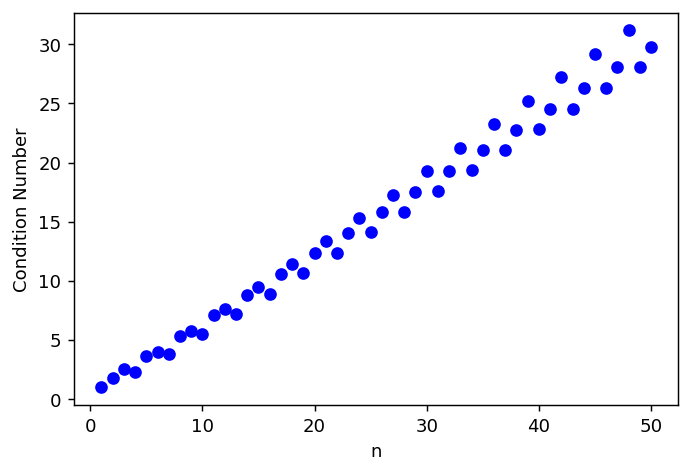
\includegraphics[width=\textwidth,height=\textheight,keepaspectratio]{cond_number.png}

\section{Observations}
The linear system presented in this exercise gets increasingly ill-conditioned as $n$ grows (as $\kappa(A_n)\geq$ for most $n$). From the plot, it can be observed that the condition number grows in a linear fashion. It can be noticed, however, that a large condition number doesn’t necessarily mean that the error will be large in all cases, just that it is possible to have a large error. The linear system appears to be ill-conditioned for most $n$ as the condition number gets increasingly bigger = than $1$. However, it can be observed that as $n$ increases, the $\widetilde{x}_1$ component gets incrementally closer to the actual $e-2$ value.\\

This error I have calculated represents how well the computed solution $\widetilde{x}_1$ approximates the true solution $x_1^{\ast}$, even though I operated in double-precision and there have been truncation errors when calculating $e-2$ and $\widetilde{x}_1$. It can be noted that the Gaussian elimination with partial pivoting doesn't introduce any additional truncation errors and therefore it is numerically stable.

\end{document}